\documentclass[UTF8]{article}
\usepackage{graphicx}
\usepackage{subfigure}
\usepackage{amsmath}
\usepackage{makecell}
\usepackage[utf8]{inputenc}
\usepackage[space]{ctex} %中文包
\usepackage{listings} %放代码
\usepackage{xcolor} %代码着色宏包
\usepackage{CJK} %显示中文宏包
\usepackage{float}

\definecolor{mygreen}{rgb}{0,0.6,0}
\definecolor{mygray}{rgb}{0.5,0.5,0.5}
\definecolor{mymauve}{rgb}{0.58,0,0.82}
\lstset{
	backgroundcolor=\color{white}, 
	basicstyle = \scriptsize,       
	breakatwhitespace = false,        
	breaklines = true,                 
	captionpos = b,                    
	commentstyle = \color{mygreen}\bfseries,
	extendedchars = false,
	frame = shadowbox, 
	framerule=0.5pt,
	keepspaces=true,
	%keywordstyle=\color{blue}\bfseries, % keyword style
	language = C++,                     % the language of code
	otherkeywords={string}, 
	numbers=left, 
	numbersep=5pt,
	numberstyle=\tiny\color{mygray},
	rulecolor=\color{black},         
	showspaces=false,  
	showstringspaces=false, 
	showtabs=false,    
	stepnumber=1,         
	%stringstyle=\color{mymauve},        % string literal style
	tabsize=4,          
	title=\lstname           
}


%画图包
\usepackage{tikz}
%画图背景包
\usetikzlibrary{backgrounds}

%自定义命令
\newcommand{\psiG}{\psi_{G}}
%在tikz中画一个顶点
%#1:node名称
%#2:位置
%#3:标签
\newcommand{\newVertex}[3]{\node[circle, draw=black, line width=1pt, scale=0.8] (#1) at #2{#3}}
%在tikz中画一条边
\newcommand{\newEdge}[2]{\draw [black,very thick](#1)--(#2)}
%在tikz中放一个标签
%#1:名称
%#2:位置
%#3:标签内容
\newcommand{\newLabel}[3]{\node[line width=1pt] (#1) at #2{#3}}


\title{中国科学技术大学计算机学院\\《计算机系统概论实验》报告}
\author{}
\date{}

\begin{document}
\maketitle
	\begin{figure}[H]
		\centering
		
\includegraphics[width=2.5in]{xiaohui.jpg}\vspace{0.5cm}\\
		\large{
			实验题目:成绩排序与统计\\
			学生姓名:王章瀚\\
			学生学号:PB18111697\\
			完成日期:\today\\
		}\vspace{2cm}
		
		%\large{计算机实验教学中心制\\2019年09月\\}
		\thispagestyle{empty}
		\clearpage  % 清除当页页码
	\end{figure}
	\newpage
	
	\section{实验要求}
	\subsection{概述}
	对60个学生的成绩进行排序,其中成绩没有相同值。在排序的基础上,对每个学生的成绩给予A/B/C/D的评价,由此统计各等级学生数量。\par
	评价标准如下:\par
	$\bullet$ 排名为前30\%,并且分数在85分以上,获A。\par
	$\bullet$ 排名为前50\%,并且分数在75分以上,获B。\par
	$\bullet$ 分数$\leq$95,获D。\par
	$\bullet$ 其他同学获C。\par
	\textbf{基本要求:}\\
	用LC-3汇编语言编写程序。程序应能够对所有分数进行排序,并计数获得A/B/C/D等级的人数。
	
	\subsection{输入与输出}
	程序输入是60个未经排序的成绩。成绩取值范围为0到100。放在从x3200开始的内存空间中,最后一个在x323B。可以认为这些成绩没有相同的。\par
	程序有两项输出:\par
	$\bullet$排序后的60的成绩。放在从x4000开始的内存空间。最高分放在x4000。
	$\bullet$获得A/B/C/D各个等级的学生数,A的放在x4100;B的放在x4101;C的放在x4102;D的放在x4103。

	\section{设计思路}
	考虑到成绩的取值范围为0到100,可以采用桶排序的思路,对每一个成绩的人数进行计数,最终能够以o(n)的时间复杂度完成任务。\par
	此外,本题题目要求中,有一个特殊点,即成绩没有重复。因此为了防止重新由内存地址算出成绩的繁琐,可以分以下两步:\par
	$\bullet$将x4000到x4064赋值为-1后,遍历x3200到x3238,直接将成绩按如下规则存储:假设当前处理的成绩为g,则将它存在\underline{x4064-g}的空间上。例如成绩100,则存放在x4000处。\par
	$\bullet$遍历x4000开始的60个成绩,将成绩前挪,消去空隙。\par
	举个例子说明(学生数为3):\par
	\begin{tabular}{|c|c|c|c|}
		\hline
		地址 & 第一步后 & 地址 & 第二步后\\
		\hline 
		x4000 & \#100 & x4000 & \#100 \\ 
		\hline 
		x4001 & \#-1 & x4000 & \#97 \\ 
		\hline 
		x4002 & \#-1 & x4000 & \#95 \\ 
		\hline 
		x4003 & \#97 & x4000 & \#-1 \\ 
		\hline 
		x4004 & \#-1 & x4000 & \#-1 \\ 
		\hline 
		x4005 & \#95 & x4000 & \#-1 \\ 
		\hline 
	\end{tabular} 
	
	\section{关键代码讲解}
	碍于篇幅原因,完整代码放在附录A中。其中代码主要分为四个部分:\par
	$\bullet$PART 1:将x4000到x4064的内存空间全部置-1。\par
	$\bullet$PART 2:遍历成绩,放到上述算法中描述的对应内存地址上。\par
	$\bullet$PART 3:对x4000到x4064中的成绩进行整理,同时统计各等级人数。\par
	$\bullet$PART 4:把剩余的空间(x403C到x4064)置0\par
	\hspace*{\fill} \\
	以下针对一些关键代码进行分析:\par
	\subsection{对于第一步的存放}
	存放过程中,由前述方法计算对应成绩应该存放的地址,用STR指令存储。\par
	寄存器使用说明:\par
	$\bullet$R1:当前正在处理的成绩的内存地址\par
	$\bullet$R2:最后一个成绩的内存地址的相反数(便于作减法)\par
	$\bullet$R3:目标地址的最后一个地址(即x4064,由x4000+\#100得到)\par
	$\bullet$R4:当前处理的成绩\par
	$\bullet$R5:临时使用\par
	\begin{lstlisting}[language=C++]
	;;;;; PART 2 ;;;;;
	; search all the grade and put them into the according memory
	; R1	grade location
	; R2	nGRADE_END
	; R3	DEST_END100	
	; R4	grade
	; R5	only for temp
				
				LD		R1, GRADE	; load the grades' address
				LD		R2, nGRADE_END	; load the opposite number of grades' end address
				LD		R3, DEST_END100	; load DEST_END100
	
	SEARCH_LOOP	LDR		R4, R1, #0	; load the grade to R4 by R1	
				NOT		R5, R4
				ADD		R5, R5, #1
				ADD		R5, R5, R3	; get the position the grade should be
				STR		R4, R5, #0	; store the grade into the position
				ADD		R1, R1, #1	; R1 ++
				ADD		R5, R1, R2	
				BRnz	SEARCH_LOOP	; check whether finished.
	\end{lstlisting}
	\subsection{对成绩对应等级的判断}
	经过排名后,可以通过存储该成绩的内存地址来判断排名,而成绩可以直接判断。有如下代码:\par
	寄存器使用说明:\par
	$\bullet$R1:将要最终存放成绩的地址\par
	$\bullet$R2:要确认是否有成绩(即不是-1)的地址\par
	$\bullet$R3:最终存放成绩的地址的相反数(即x4064,由x4000+\#100得到)\par
	$\bullet$R4:当前处理的成绩\par
	$\bullet$R5:临时使用\par
	\begin{lstlisting}[language=C++]
	;;;;; PART 3 ;;;;;
	; put the grades into the corret positions
	; R1	destination
	; R2	to find next filled memory
	; R3	nDEST_END
	; R4	grade
	; R5	only for temp 
	
	; try A
				LD		R5, A_GRADE	
				NOT		R5, R5
				ADD		R5, R5, #1
				ADD		R5, R4, R5	; R5 <- (R4-A_GRADE) 
				BRn		NOTA		; if(R4 < A_GRADE) goto NOTA
				LD		R5, A_RANK
				NOT		R5, R5
				ADD		R5, R5, #1
				ADD		R5, R1, R5	; R5 <- (R1-A_RANK) 
				BRp		NOTA		; else if(R5 > 0) goto NOTA
				LDI		R5, As		; load the address of statistics information.
				ADD		R5, R5, #1	; As++
				STI		R5, As
				BRnzp	LOOP_PRE
	\end{lstlisting}
	
	\section{调试分析}
	由于设计的各种数值较多,导致编写代码时有些混乱。经过逐步调试,最终纠正过来。\par
	
	\section{代码测试}
	为测试代码,编写了生成测试数据的代码。(见附录B)\par
	\subsection{测试数据1}
	\begin{lstlisting}[language=C++]
		.ORIG		x3200
		.FILL		#50
		.FILL		#1
		.FILL		#32
		.FILL		#41
		.FILL		#88
		;... here skipped some
		.FILL		#24
		.FILL		#52
		.FILL		#54
		.FILL		#40
		.FILL		#14
		.END
	; As:9	Bs:5	Cs:6	Ds40
	\end{lstlisting}
	
	\begin{figure}[H]
		\begin{minipage}[H]{0.48\linewidth}
			\centering
			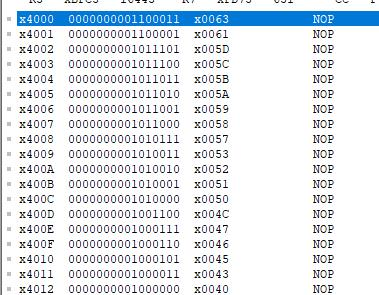
\includegraphics[scale=0.45]{1_1.jpg}
			\caption{排序结果部分截图}
			\label{1_1}
		\end{minipage}
		\begin{minipage}[H]{0.48\linewidth}
			\centering
			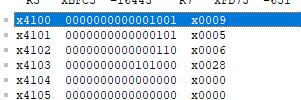
\includegraphics[scale=0.4]{1_2.jpg}
			\caption{统计结果截图}
			\label{1_2}
		\end{minipage}
	\end{figure}


	\subsection{测试数据2}
	\begin{lstlisting}[language=C++]
		.ORIG		x3200
		.FILL		#41
		.FILL		#67
		.FILL		#58
		.FILL		#14
		.FILL		#26
		;... here skipped some
		.FILL		#62
		.FILL		#27
		.FILL		#6
		.FILL		#28
		.FILL		#90
		.END
	; As:10	Bs:6	Cs:11	Ds33
	
	\end{lstlisting}
	
	\begin{figure}[H]
		\begin{minipage}[H]{0.48\linewidth}
			\centering
			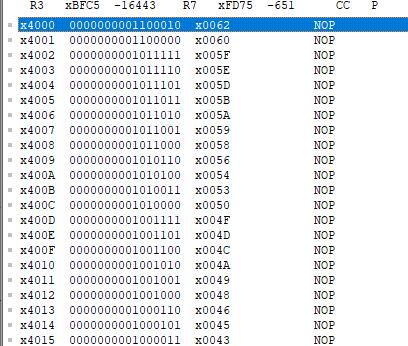
\includegraphics[scale=0.45]{2_1.jpg}
			\caption{排序结果部分截图}
			\label{2_1}
		\end{minipage}
		\begin{minipage}[H]{0.48\linewidth}
			\centering
			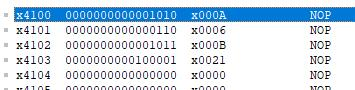
\includegraphics[scale=0.4]{2_2.jpg}
			\caption{统计结果截图}
			\label{2_2}
		\end{minipage}
	\end{figure}

	\section{实验总结}
	本次实验中,经过一系列的编程练习,我对于LC-3的汇编代码更加熟悉,同时也能够熟练使用对应Simulator。\par
	此外,初见题目便匆忙开始写代码,没有过多的分析,最终使用了选择排序这样的代码来完成题目,虽然也能完成,但执行指令数(平均在40000左右)相对于用现在的算法的指令数(2800左右)较多。经过思考,修改方案为桶排序,并进行一定程度的改进,最终有了上述结果。因此本次实验的一个较大收获是,它让我明白了分析的重要性,而不应拿到一个任务就急忙上手。\par
	
	
	\section{附录}
	\subsection{附录A}
	
	\begin{lstlisting}[language=C++]
				.ORIG		x3000		; start from x3000
	
	;;;;; PART 1 ;;;;;
	; make the destination memory into 0, from DEST to DEST_END
	; R1	DEST
	; R2	nDEST_END100
	; R3	-1
	
				LD		R1, DEST
				LD		R2, nDEST_END100
				AND		R3, R3, #0
				ADD		R3, R3, #-1
	SETn1_LOOP	STR		R3, R1, #0	; store 0 into the position
				ADD		R1, R1, #1	; R1 ++
				ADD		R5, R1, R2	
				BRnz	SETn1_LOOP	; check whether finished.
	
	;;;;; PART 2 ;;;;;
	; search all the grade and put them into the according memory
	; R1	grade location
	; R2	nGRADE_END
	; R3	DEST_END100	
	; R4	grade
	; R5	only for temp
	
				LD		R1, GRADE	; load the grades' address
				LD		R2, nGRADE_END	; load the opposite number of grades' end address
				LD		R3, DEST_END100	; load DEST_END100
	
	SEARCH_LOOP	LDR		R4, R1, #0	; load the grade to R4 by R1	
				NOT		R5, R4
				ADD		R5, R5, #1
				ADD		R5, R5, R3	; get the position the grade should be
				STR		R4, R5, #0	; store the grade into the position
				ADD		R1, R1, #1	; R1 ++
				ADD		R5, R1, R2	
				BRnz	SEARCH_LOOP	; check whether finished.	
	
	;;;;; PART 3 ;;;;;
	; put the grades into the corret positions
	; R1	destination
	; R2	to find next filled memory
	; R3	nDEST_END
	; R4	grade
	; R5	only for temp 
				LD		R1, DEST
				LD		R2, DEST
				LD		R3, nDEST_END
				
	SORT_LOOP	ADD		R2, R2, #1	
				LDR		R4, R2, #-1	; load the grade to R4 by R2
				BRn		SORT_LOOP	; if the grade is negative(-1), take next
	
	; else find the A/B/C/D for this grade.
	; try A
				LD		R5, A_GRADE	
				NOT		R5, R5
				ADD		R5, R5, #1
				ADD		R5, R4, R5	; R5 <- (R4-A_GRADE) 
				BRn		NOTA		; if(R4 < A_GRADE) goto NOTA
				LD		R5, A_RANK
				NOT		R5, R5
				ADD		R5, R5, #1
				ADD		R5, R1, R5	; R5 <- (R1-A_RANK) 
				BRp		NOTA		; else if(R5 > 0) goto NOTA
				LDI		R5, As		; load the address of statistics information.
				ADD		R5, R5, #1	; As++
				STI		R5, As
				BRnzp	LOOP_PRE	
	; else try B
	NOTA		LD		R5, B_GRADE	
				NOT		R5, R5
				ADD		R5, R5, #1
				ADD		R5, R4, R5	; R5 <- (R4-B_GRADE) 
				BRn		NOTB		; if(R4 < B_GRADE) goto NOTB
				LD		R5, B_RANK
				NOT		R5, R5
				ADD		R5, R5, #1
				ADD		R5, R1, R5	; R5 <- (R1-B_RANK) 
				BRp		NOTA		; else if(R5 > 0) goto NOTB
				LDI		R5, Bs		; load the address of statistics information.
				ADD		R5, R5, #1	; Bs++
				STI		R5, Bs		; store the new Bs
				BRnzp	LOOP_PRE	
	; else try D
	NOTB		LD		R5, D_GRADE	
				NOT		R5, R5
				ADD		R5, R5, #1
				ADD		R5, R4, R5	; R5 <- (R4-D_GRADE) 
				BRp		NOTD		; if(R4 < D_GRADE) goto NOTD
				LDI		R5, Ds		; load the address of statistics information.
				ADD		R5, R5, #1	; Ds++
				STI		R5, Ds		; store the new Ds
				BRnzp	LOOP_PRE	
	; else, C
	NOTD		LDI		R5, Cs		; load the address of statistics infsormation.
				ADD		R5, R5, #1	; Cs++
				STI		R5, Cs		; store the new Cs
	
	; above finished get the A/B/C/D
	LOOP_PRE	STR		R4, R1, #0	; store the grade to the correct position
				ADD		R1, R1, #1	; R1++
				ADD		R5, R3, R1
				BRnz	SORT_LOOP	; 
	
	;;;;; PART 4 ;;;;;
	; clear the following into 0
	; R1	destination
	; R2	nDEST_END100
	; R4	0
	
				LD		R2, nDEST_END100
				AND		R4, R4, #0
	SET0_LOOP	STR		R4, R1, #0	; store 0 into the position
				ADD		R1, R1, #1	; R1 ++
				ADD		R5, R1, R2	
				BRnz	SET0_LOOP	; check whether finished.
	
				HALT
	
	A_GRADE		.FILL		85		; the least grade requirement for A
	B_GRADE		.FILL		75		; the least grade requirement for B
	D_GRADE		.FILL		59		; the grade requirement for D
	A_RANK		.FILL		x4011	; the rank requirement for A. 
	B_RANK		.FILL		x401C	; the rank requirement for B. 
	
	GRADE		.FILL		x3200	; the start address of grades
	nGRADE_END	.FILL		x-323B	; the opposite number of end address of grades
	DEST		.FILL		x4000	; the start address of grades
	DEST_END100	.FILL		x4064	; the end address of destination.
	nDEST_END100.FILL		x-4064	; the opposite number of end address of destination.
	nDEST_END	.FILL		x-403B	; the opposite number of end address of destination.
	As			.FILL		x4100	; the address of number of As.
	Bs			.FILL		x4101	; the address of number of Bs.
	Cs			.FILL		x4102	; the address of number of Cs.
	Ds			.FILL		x4103	; the address of number of Ds.
	
				.END
	\end{lstlisting}

	\subsection{附录B}
	\begin{lstlisting}[language=C++]
	#include <iostream>
	#include <algorithm>
	#include <cstdlib>
	#include <ctime>
	using namespace std;
	
	int cmp(int a, int b){
		return b < a;
	}
	
	int main() {
		FILE* f = fopen("data.asm", "w");
		srand((unsigned)time(NULL)); //将系统时间作为随机种子 
		int n, temp;
		cin >> n;
		int* scores = new int(n);
		fprintf(stdout, "\t.ORIG\t\tx3200\n");
		fprintf(f, "\t.ORIG\t\tx3200\n");
		for(int i = 0; i < n; i++){
			temp = rand()%100;
			bool flag = 1;
			while(flag) {
				int j;
				for(j = 0; j < i; j++) {
					if(scores[j] == temp){
						temp = rand()%100;
						break;
					}
				}
				if(j == i)
					flag = 0;
			}
			scores[i] = temp;
			fprintf(stdout, "\t.FILL\t\t#%d\n", temp);
			fprintf(f, "\t.FILL\t\t#%d\n", temp);
		}
		fprintf(f, "\t.END\n");
		fprintf(stdout, "\t.END\n");
		
		int grades[4] = {0};
		sort(scores, scores+n, cmp);
		for(int i = 0; i < n; i++){
			if(scores[i] >= 75) {
				if(scores[i] >= 85 && i < n*0.3)
					grades[0]++;
				else if(i < n*0.5)
					grades[1]++;
			}
			else if(scores[i] < 60)
				grades[3]++;
			else
				grades[2]++;
			printf("%x\n", scores[i]);
		}
		fprintf(f, "; As:%d\tBs:%d\tCs:%d\tDs%d\n", grades[0], grades[1], grades[2], grades[3]);
		fprintf(stdout, "; As:%d\tBs:%d\tCs:%d\tDs%d\n", grades[0], grades[1], grades[2], grades[3]);
		fclose(f);
	}
	\end{lstlisting}

\end{document}
